\documentclass[12pt, a4paper, simple]{eskdtext}

\usepackage{hyperref}
\usepackage{env}
\usepackage{_sty/gpi_lst}
\usepackage{_sty/gpi_toc}
\usepackage{_sty/gpi_t}
\usepackage{_sty/gpi_p}
\usepackage{_sty/gpi_u}

% Код
\ESKDletter{}{К}{П}
\def \gpiDocTypeNum {81}
\def \gpiCode {\ESKDtheLetterI\ESKDtheLetterII\ESKDtheLetterIII.\gpiStudentGroupName\gpiStudentGroupNum.\gpiStudentCard~-~0\gpiDocNum~\gpiDocTypeNum~\gpiDocVersion}

\def \gpiDocTopic {ПОЯСНИТЕЛЬНАЯ ЗАПИСКА К КУРСОВОМУ ПРОЕКТУ}

% Графа 1 (наименование изделия/документа)
\ESKDcolumnI {\ESKDfontII \gpiTopic \\ \gpiDocTopic}

% Графа 2 (обозначение документа)
\ESKDsignature {\gpiCode}

% Графа 9 (наименование или различительный индекс предприятия) задает команда
\ESKDcolumnIX {\gpiDepartment}

% Графа 11 (фамилии лиц, подписывающих документ) задают команды
\ESKDcolumnXIfI {\gpiStudentSurname}
\ESKDcolumnXIfII {\gpiTeacherSurname}
\ESKDcolumnXIfV {\gpiTeacherSurname}

\begin{document}
    \begin{ESKDtitlePage}
    \begin{center}
        \gpiMinEdu \\
        \gpiEdu \\
        \gpiKaf \\
    \end{center}

    \vfill

    \begin{center}
        \gpiTopic \\
    \end{center}

    \vfill

    \begin{center}
        \textbf{\gpiDocTopic} \\
        ПО ДИСЦИПЛИНЕ \gpiDiscipline \\
    \end{center}

    \vfill

    \begin{center}
        \gpiCode \\
        Листов \pageref{LastPage} \\
    \end{center}

    \vfill

    \begin{flushright}
        \begin{minipage}[t]{.49\textwidth}
            \begin{minipage}[t]{.75\textwidth}
                \begin{flushright}
                    Руководитель

                    Выполнил

                    Консультант

                    по ЕСПД
                \end{flushright}
            \end{minipage}
        \end{minipage}
        \begin{minipage}[t]{.49\textwidth}
            \begin{flushright}
                \begin{minipage}[t]{.75\textwidth}
                    \gpiTeacherName~\gpiTeacherSurname

                    \gpiStudentName~\gpiStudentSurname

                    \hspace{0pt}

                    \gpiTeacherName~\gpiTeacherSurname

                \end{minipage}
            \end{flushright}
            
        \end{minipage}
    \end{flushright}

    \vfill

    \begin{center}
        \ESKDtheYear
    \end{center}
\end{ESKDtitlePage}


    \ESKDthisStyle{empty}
    лист с заданием
    \newpage

    % Содержание
    \ESKDthisStyle{formII}
    \tableofcontents
    \thispagestyle{toc}
    \pagestyle{toc}
    \hspace{0pt}\\
    ПРИЛОЖЕНИЕ А. НАБОР ТЕСТОВЫХ ЗАДАНИЙ ДЛЯ ПРОВЕРКИ\\
    ПРИЛОЖЕНИЕ Б. РЕЗУЛЬТАТЫ СОЗДАНИЯ, ЗАГРУЗКИ И ПРОВЕРКИ БД\\
    \newpage

    %
    \newpage
    \addcontentsline{toc}{section}{ВВЕДЕНИЕ}
    \section*{ВВЕДЕНИЕ}
    \newpage

    %
    \section{ОПИСАНИЕ МОДЕЛИ АВТОМАТИЗАЦИИ}
    \subsection{Организационная модель}

    Организационная структура - совокупность подразделений организации и их взаимосвязей,
    в рамках которой между подразделениями распределяются функциональные задачи,
    определяются полномочия и ответственность руководителей и должностных лиц.
    
    Структура предприятия устанавливается исходя из объема и содержания задач,
    решаемых предприятием, направленности и интенсивности сложившихся на предприятии
    информационных и документационных потоков и с учетом его организационных и материальных возможностей.

    Оргструктура представляется через органограмму и такие документы, как штатное расписание,
    устав организации и пр.

    Органограмма - графическое представление структуры организации.

    Организационная модель ОА <<Косметический салон>> представлена органограммой <<Косметический салон>>
    на рис.~\ref{fig:OrganizationnayModel}
    с использованием нотации Organizational chart методологии ARIS,
    а также таблицей <<Каталог организационных единиц>>
    на рис.~\ref{fig:OrganizationnieEdinici_katalog}.

    \begin{figure}[!h]
        \centering
        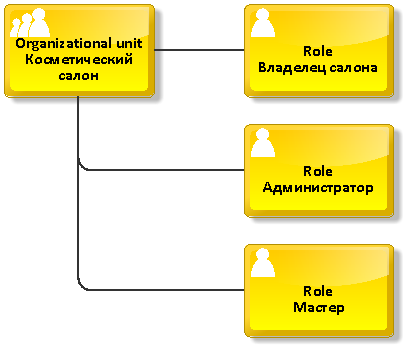
\includegraphics[height=6cm]
            {_docs/ОрганизационнаяМодель.png}
        \caption{Органограмма ОА <<Косметический салон>>}
        \label{fig:OrganizationnayModel}
    \end{figure}

    \begin{figure}[!h]
        \centering
        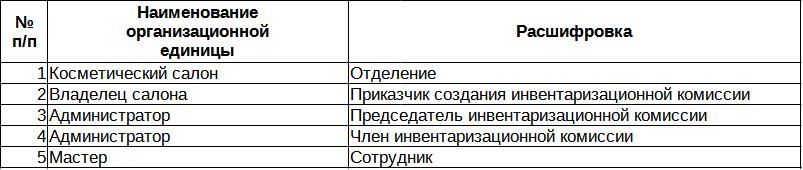
\includegraphics[width=16cm]
            {_docs/ОрганизационныеЕдиницы_каталог.jpg}
        \caption{Каталог организационых единиц}
        \label{fig:OrganizationnieEdinici_katalog}
    \end{figure}

    \subsection{Функциональная модель}

    Функциональная модель объекта автоматизации - описание его на языке выполняемых функций и их отношений.
    Функциональная структура - структура, элементами которой являются функции,
    реализуемые подразделениями предприятия, а отношениями являются связи,
    обеспечивающие передачу между элементами предметов труда.
    Функция – это предметно-ориентированное задание или действие,
    в результате которой выполняется одна или несколько целей, стоящих перед компанией.
    Функции предприятия распределяются по компонентам оргструктуры и представляют собой иерархическое дерево,
    строящееся от общего к частному.
    На самом верхнем уровне описываются самые сложные функции,
    которые потом детализируются через свои функциональные составляющие.

    Функциональная модель ОА <<Косметический салон>> представлена
    на рис.~\ref{fig:FynctionalnayModel}
    с использованием нотации Process landscape методологии ARIS,
    а также таблицей <<Каталог функций>>
    на рис.~\ref{fig:Fynctii_katalog}.

    \begin{figure}[!h]
        \centering
        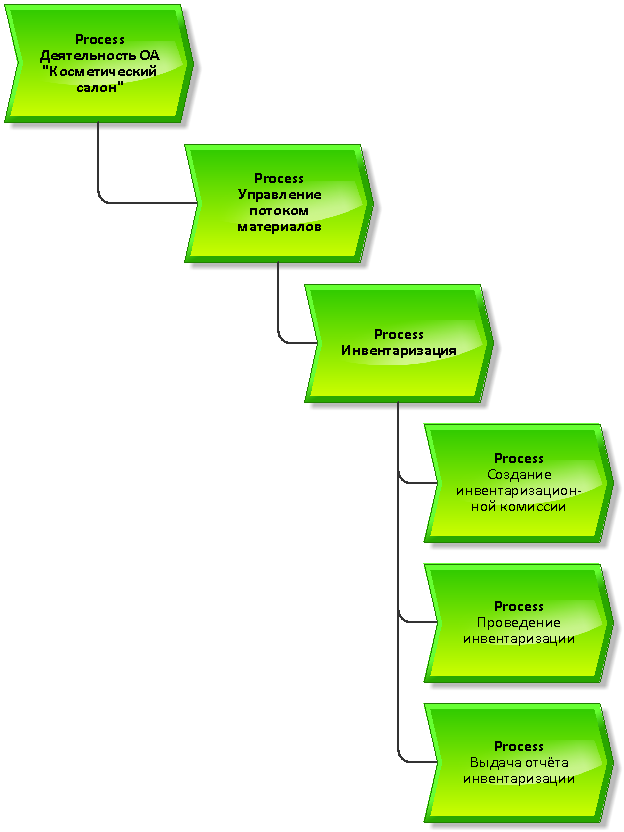
\includegraphics[height=8cm]
            {_docs/ФункциональнаяМодель.png}
        \caption{Функциональное дерево ОА "Косметический салон"}
        \label{fig:FynctionalnayModel}
    \end{figure}

    \begin{figure}[!h]
        \centering
        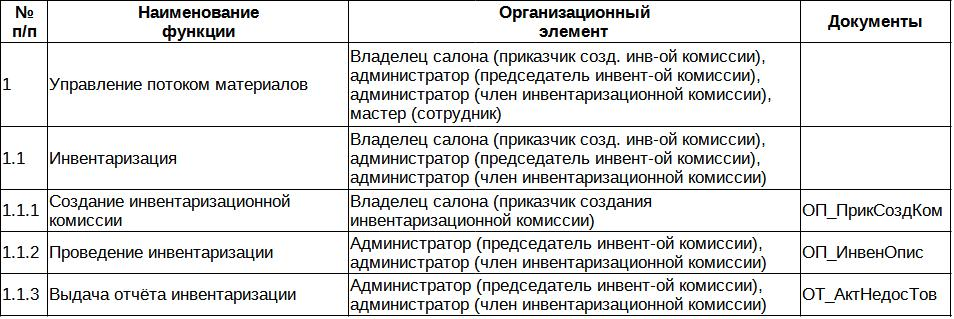
\includegraphics[width=12cm]
            {_docs/Функции_каталог.jpg}
        \caption{Каталог функций}
        \label{fig:Fynctii_katalog}
    \end{figure}

    \newpage
    \subsection{Информационная модель}
    Информационная модель - модель объекта, представленная в виде информации,
    описывающей существенные для данного рассмотрения параметры и переменные величины объекта,
    связи между ними, входы и выходы объекта и позволяющая путём подачи на модель информации об изменениях
    входных величин моделировать возможные состояния объекта.

    Информационная модель ОА <<Инвентаризация>> для ИС <<Косметический салон>> включает в себя следующие документы:

    \begin{enumerate}
        \item[1.] Справочные документы (рисунок~\ref{fig:CP_katalog}).
        \item[2.] Оперативные документы (рисунок~\ref{fig:OP_katalog}).
        \item[3.] Отчётные документы (рисунок~\ref{fig:OT_katalog}).
    \end{enumerate}

    % Справочные документы представлены в <<Каталоге справочных документов>> .

    \begin{figure}[!h]
        \centering
        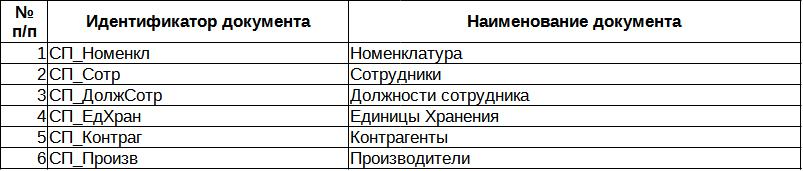
\includegraphics[width=14cm]
            {_docs/СП_каталог.jpg}
        \caption{Каталог справочных документов}
        \label{fig:CP_katalog}
    \end{figure}

    % Оперативные документы представлены в <<Каталоге оперативных документов>> .
    
    \begin{figure}[!h]
        \centering
        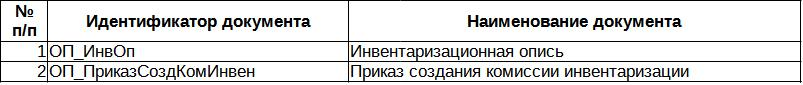
\includegraphics[width=14cm]
            {_docs/ОП_каталог.jpg}
        \caption{Каталог оперативных документов}
        \label{fig:OP_katalog}
    \end{figure}

    % Отчётные документы представлены в <<Каталоге отчётных документов>> .
    
    \begin{figure}[!h]
        \centering
        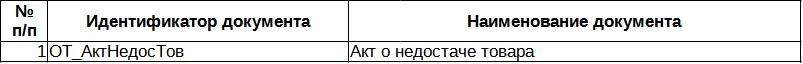
\includegraphics[width=14cm]
            {_docs/ОТ_каталог.jpg}
        \caption{Каталог отчётных документов}
        \label{fig:OT_katalog}
    \end{figure}

    \newpage

    \subsubsection{Справочные документы}

    \paragraph{} \textbf{Справочник <<Номенклатура>>}

    Справочник <<Номенклатура>> - содержит информацию о материалах.
    Документ представлен в виде словаря данных (рисунок~\ref{fig:CP_Nomenkl_tipi})
    и макета (рисунок~\ref{fig:CP_Nomenkl_maket}).

    \begin{figure}[!h]
        \centering
        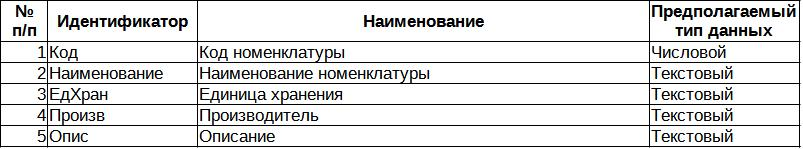
\includegraphics[width=14cm]
            {_docs/СП_Номенкл_типы.jpg}
        \caption{Словарь данных справочника <<Номеклатура>>}
        \label{fig:CP_Nomenkl_tipi}
    \end{figure}

    \begin{figure}[!h]
        \centering
        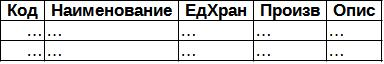
\includegraphics[]
            {_docs/СП_Номенкл_макет.jpg}
        \caption{Макет справочника <<Номеклатура>>}
        \label{fig:CP_Nomenkl_maket}
    \end{figure}

    \paragraph{} \textbf{Справочник <<Сотрудники>>}

    Справочник <<Сотрудники>> - содержит информацию о сотрудниках.
    Документ представлен в виде словаря данных (рисунок~\ref{fig:CP_Sotr_tipi})
    и макета (рисунок~\ref{fig:CP_Sotr_maket}).

    \begin{figure}[!h]
        \centering
        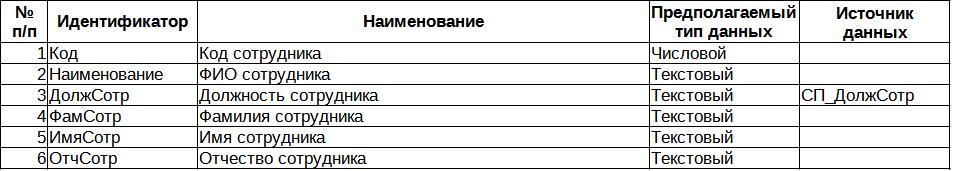
\includegraphics[width=14cm]
            {_docs/СП_Сотр_типы.jpg}
        \caption{Словарь данных справочника <<Сотрудники>>}
        \label{fig:CP_Sotr_tipi}
    \end{figure}

    \begin{figure}[!h]
        \centering
        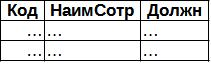
\includegraphics[]
            {_docs/СП_Сотр_макет.jpg}
        \caption{Макет справочника <<Сотрудники>>}
        \label{fig:CP_Sotr_maket}
    \end{figure}

    \newpage

    \paragraph{} \textbf{Справочник <<Должности сотрудника>>}

    Справочник <<Должности сотрудника>> - содержит перечисления должностей сотрудника.
    Документ представлен в виде словаря данных (рисунок~\ref{fig:CP_DoljnCotr_tipi})
    и макета (рисунок~\ref{fig:CP_DoljnCotr_maket}).

    \begin{figure}[!h]
        \centering
        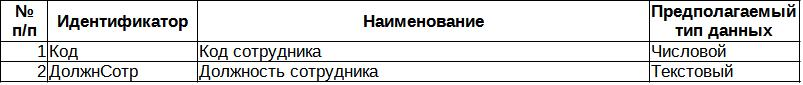
\includegraphics[width=14cm]
            {_docs/СП_ДолжнСотр_типы.jpg}
        \caption{Словарь данных справочника <<Должности сотрудника>>}
        \label{fig:CP_DoljnCotr_tipi}
    \end{figure}

    \begin{figure}[!h]
        \centering
        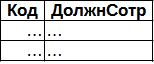
\includegraphics[]
            {_docs/СП_ДолжнСотр_макет.jpg}
        \caption{Макет справочника <<Должности сотрудника>>}
        \label{fig:CP_DoljnCotr_maket}
    \end{figure}

    \paragraph{} \textbf{Справочник <<Единицы хранения>>}

    Справочник <<Единицы хранения>> - содержит перечисление единиц хранения.
    Документ представлен в виде словаря данных (рисунок~\ref{fig:CP_EdXran_tipi})
    и макета (рисунок~\ref{fig:CP_EdXran_maket}).

    \begin{figure}[!h]
        \centering
        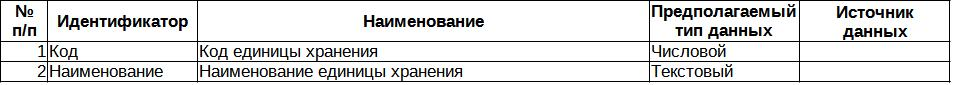
\includegraphics[width=14cm]
            {_docs/СП_ЕдХран_типы.jpg}
        \caption{Словарь данных справочника <<Единицы хранения>>}
        \label{fig:CP_EdXran_tipi}
    \end{figure}

    \begin{figure}[!h]
        \centering
        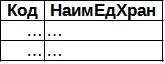
\includegraphics[]
            {_docs/СП_ЕдХран_макет.jpg}
        \caption{Макет справочника <<Единицы хранения>>}
        \label{fig:CP_EdXran_maket}
    \end{figure}

    \newpage

    \paragraph{} \textbf{Справочник <<Мои организации>>}

    Справочник <<Мои организации>> - содержит информацию о моих организациях.
    Документ представлен в виде словаря данных (рисунок~\ref{fig:CP_MoiOrg_tipi})
    и макета (рисунок~\ref{fig:CP_MoiOrg_maket}).

    \begin{figure}[!h]
        \centering
        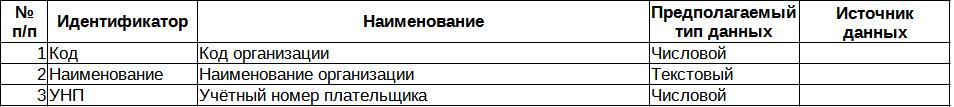
\includegraphics[width=14cm]
            {_docs/СП_МоиОрг_типы.jpg}
        \caption{Словарь данных справочника <<Мои организации>>}
        \label{fig:CP_MoiOrg_tipi}
    \end{figure}

    \begin{figure}[!h]
        \centering
        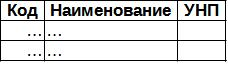
\includegraphics[]
            {_docs/СП_МоиОрг_макет.jpg}
        \caption{Макет справочника <<Мои организации>>}
        \label{fig:CP_MoiOrg_maket}
    \end{figure}

    \paragraph{} \textbf{Справочник <<Производители>>}

    Справочник <<Производители>> - содержит перечисление производителей.
    Документ представлен в виде словаря данных (рисунок~\ref{fig:CP_Proizv_tipi})
    и макета (рисунок~\ref{fig:CP_Proizv_maket}).

    \begin{figure}[!h]
        \centering
        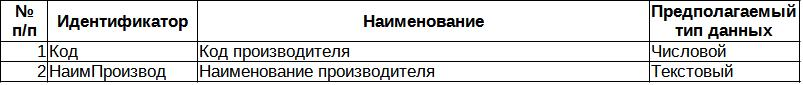
\includegraphics[width=14cm]
            {_docs/СП_Произв_типы.jpg}
        \caption{Словарь данных справочника <<Производители>>}
        \label{fig:CP_Proizv_tipi}
    \end{figure}

    \begin{figure}[!h]
        \centering
        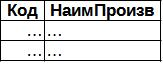
\includegraphics[]
            {_docs/СП_Произв_макет.jpg}
        \caption{Макет справочника <<Производители>>}
        \label{fig:CP_Proizv_maket}
    \end{figure}

    \newpage

    \subsubsection{Оперативные документы}

    \paragraph{} \textbf{Оперативный документ <<Инвентаризационная опись>>}

    Оперативный документ <<Инвентаризационная опись>>
    - документ, в котором отображаются результаты инвентаризации.
    Документ представлен в виде словаря данных (рисунок~\ref{fig:OP_InvenOpis_tipi})
    и макета (рисунок~\ref{fig:OP_InvenOpis_maket}).

    \begin{figure}[!h]
        \centering
        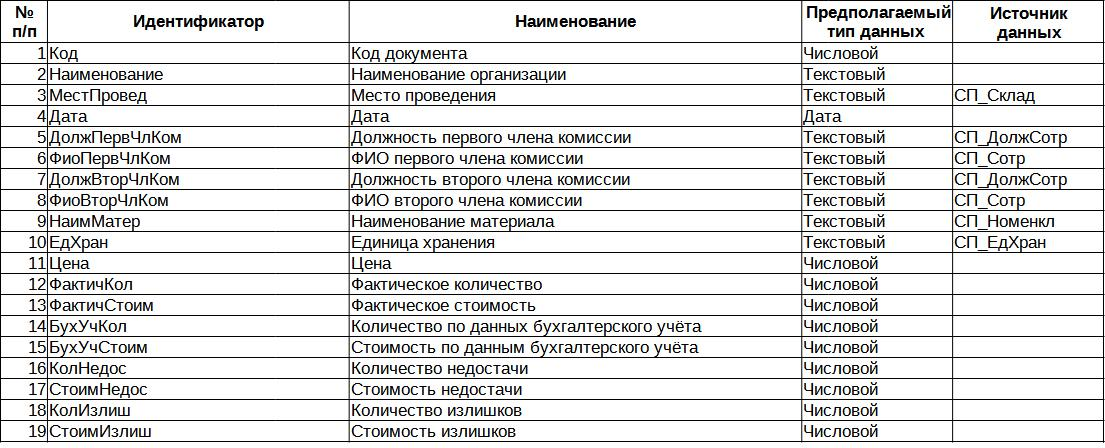
\includegraphics[width=14cm]
            {_docs/ОП_ИнвенОпис_типы.jpg}
        \caption{Словарь данных документа <<Инвентаризационная опись>>}
        \label{fig:OP_InvenOpis_tipi}
    \end{figure}

    \begin{figure}[!h]
        \centering
        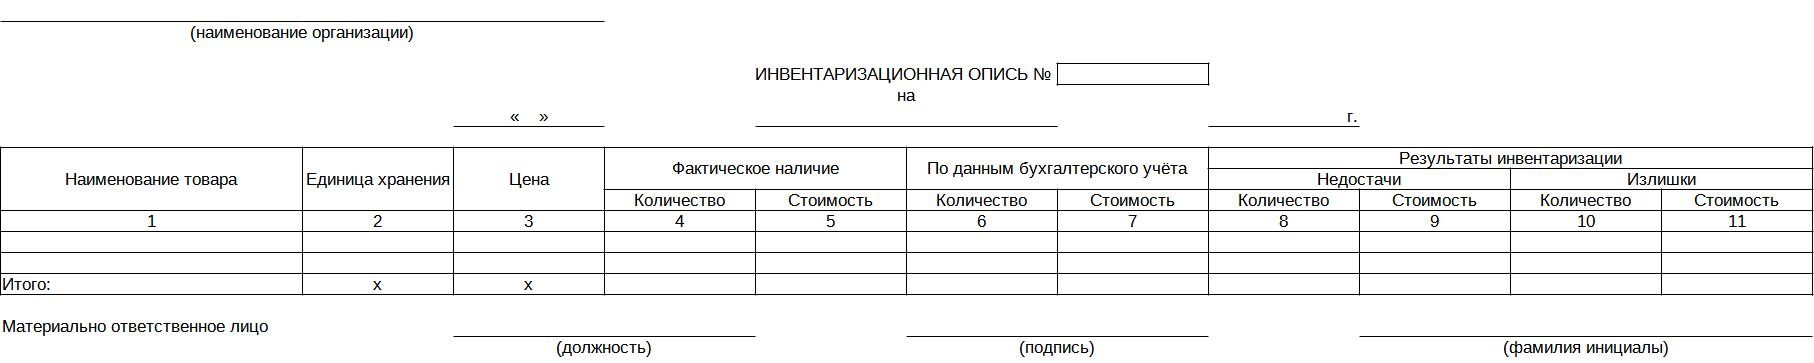
\includegraphics[width=14cm]
            {_docs/ОП_ИнвенОпис_макет.jpg}
        \caption{Макет документа <<Инвентаризационная опись>>}
        \label{fig:OP_InvenOpis_maket}
    \end{figure}

    \begin{figure}[!h]
        \centering
        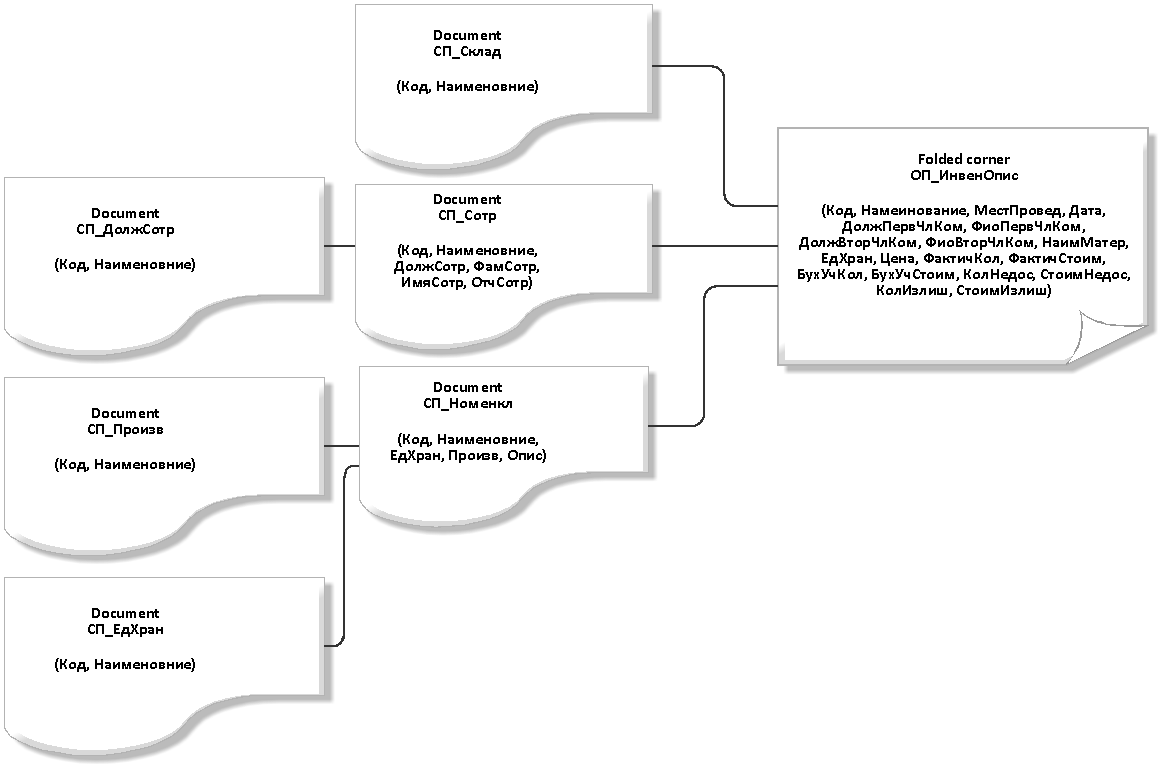
\includegraphics[height=7cm]
            {_docs/ОП_ИнвенОпис_связи.png}
        \caption{Схема информационной связи документа <<Инвентаризационная опись>>}
        \label{fig:OP_InvenOpis_svazi}
    \end{figure}

    \newpage
    \paragraph{} \textbf{Оперативный документ <<Приказ о создании инвентаризационной комиссии>>}

    Оперативный документ <<Приказ о создании инвентаризационной комиссии>>
    - документ, который формируется перед инвентаризацией товара.
    Документ представлен в виде словаря данных (рисунок~\ref{fig:OP_PrikazSozdKomInvest_tipi})
    и макета (рисунок~\ref{fig:OP_PrikazSozdKomInvest_maket}).

    \begin{figure}[!h]
        \centering
        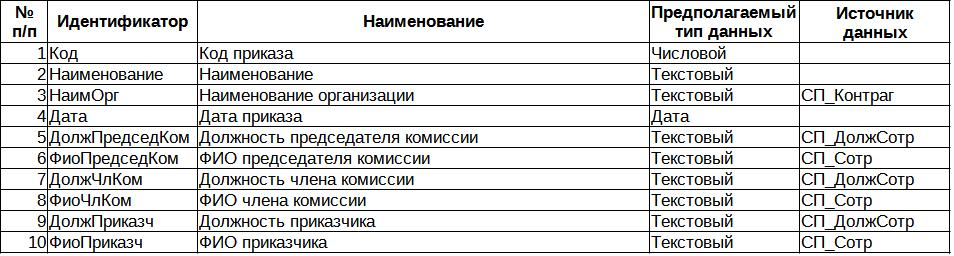
\includegraphics[width=14cm]
            {_docs/ОП_ПриказСоздКомИнвент_типы.jpg}
        \caption{Словарь данных документа <<Приказ о создании инвентаризационной комиссии>>}
        \label{fig:OP_PrikazSozdKomInvest_tipi}
    \end{figure}

    \begin{figure}[!h]
        \centering
        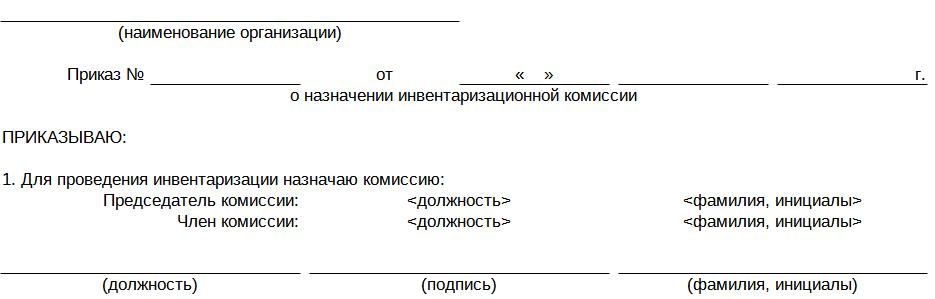
\includegraphics[width=14cm]
            {_docs/ОП_ПриказСоздКомИнвент_макет.jpg}
        \caption{Макет документа <<Приказ о создании инвентаризационной комиссии>>}
        \label{fig:OP_PrikazSozdKomInvest_maket}
    \end{figure}

    \begin{figure}[!h]
        \centering
        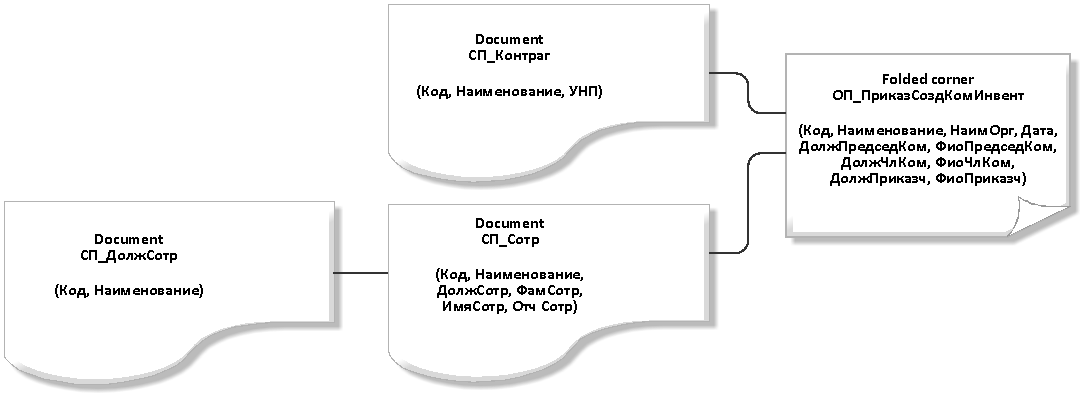
\includegraphics[height=6cm]
            {_docs/ОП_ПриказСоздКомИнвент_связи.png}
        \caption{Схема информационной связи документа <<Приказ о создании инвентаризационной комиссии>>}
        \label{fig:OP_PrikazSozdKomInvest_svazi}
    \end{figure}

    \newpage
    \subsubsection{Отчётные документы}

    \paragraph{} \textbf{Отчётный документ <<Акт о нестаче товара>>}

    Отчётный документ <<Акт о нестаче товара>>
    - формируется после проведения инвентаризации.
    Документ представлен в виде словаря данных (рисунок~\ref{fig:OT_AktNedosTov_tipi})
    и макета (рисунок~\ref{fig:OT_AktNedosTov_maket}).

    \begin{figure}[!h]
        \centering
        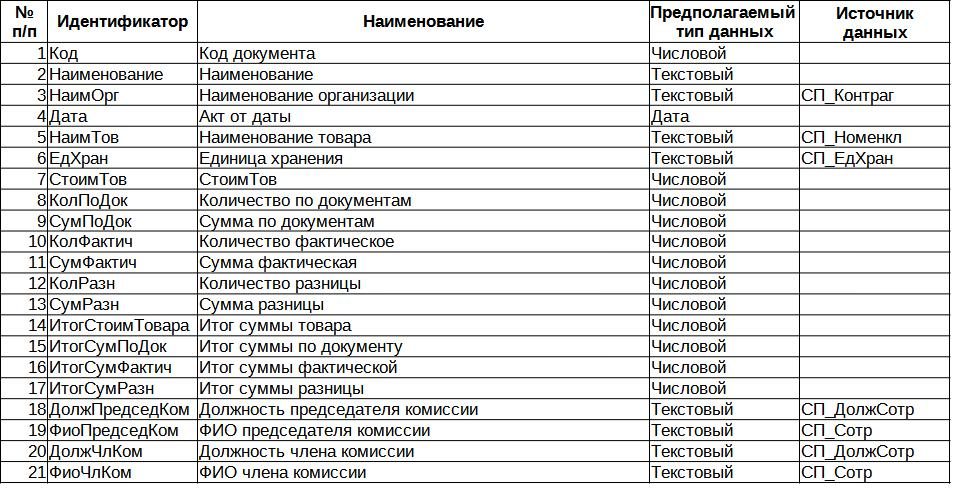
\includegraphics[width=14cm]
            {_docs/ОТ_АктНедосТов_типы.jpg}
        \caption{Словарь данных документа <<Акт о нестаче товара>>}
        \label{fig:OT_AktNedosTov_tipi}
    \end{figure}

    \begin{figure}[!h]
        \centering
        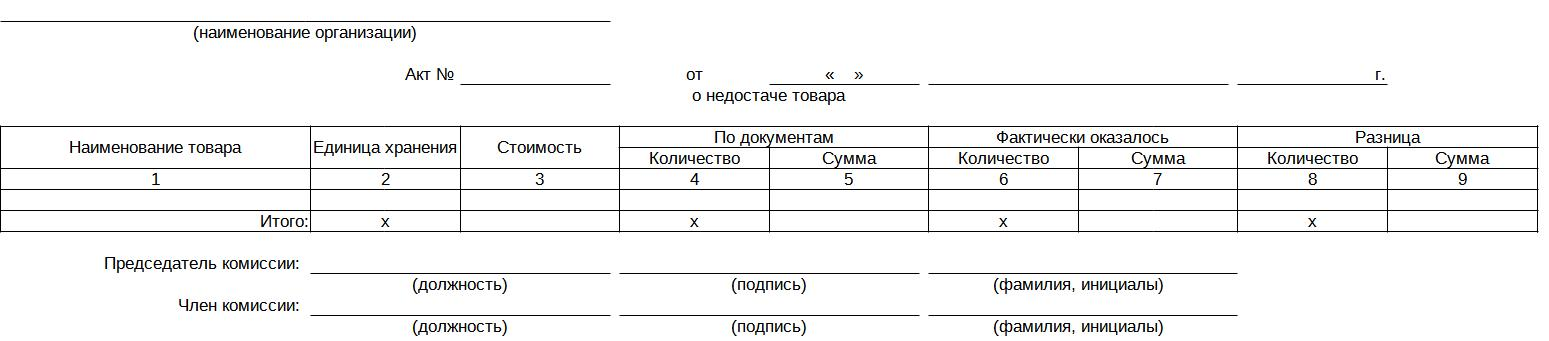
\includegraphics[width=14cm]
            {_docs/ОТ_АктНедосТов_макет.jpg}
        \caption{Макет документа <<Акт о нестаче товара>>}
        \label{fig:OT_AktNedosTov_maket}
    \end{figure}

    \begin{figure}[!h]
        \centering
        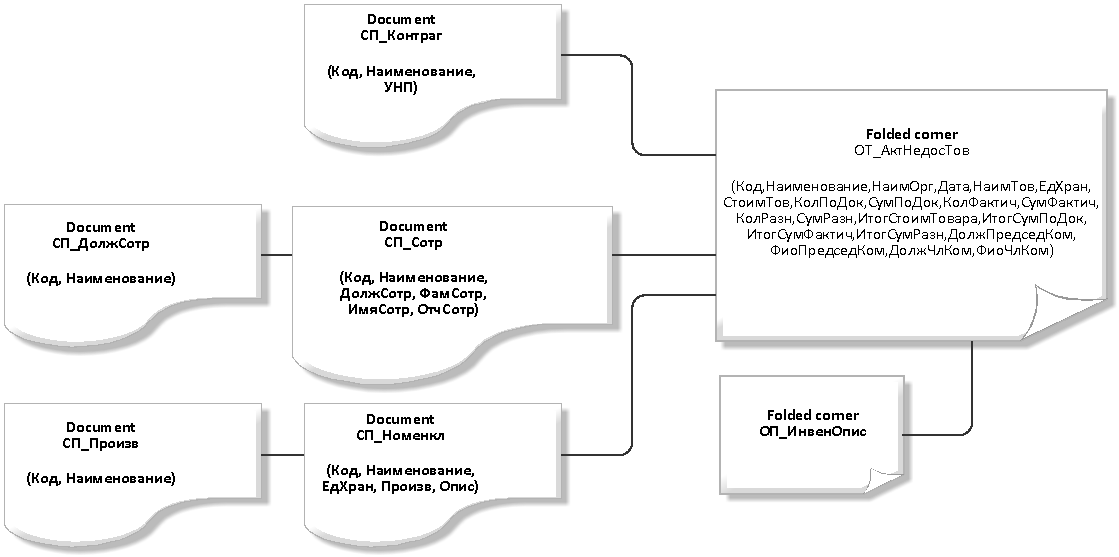
\includegraphics[height=6cm]
            {_docs/ОТ_АктНедосТов_связи.png}
        \caption{Схема информационной связи документа <<Акт о нестаче товара>>}
        \label{fig:OP_AktNedosTov_svazi}
    \end{figure}

    \newpage
    \subsection{Модель бизнес-процесса объекта автоматизации}

    Процесс - любая деятельность, в которой используются ресурсы для преобразования входов в выходы.
    Зачастую представляет из себя совокупность взаимосвязанных и совершенных работ,
    в которых результаты одной работы являются началом другой работы,
    образуя цепочку внутрненних поставщиков и потребителей.

    Бизнес-процесс - устойчивая и целенаправленная совокупность взаимосвязанных видов деятельности,
    которая по определённой технологии преобразует входной сигнал в выходной, представляющий ценность для потребителя.

    eEPC - нотация для проектирования бизнес-процессов.
    Данная нотация ARIS представляет бизнес-процесс как цепочку событий и действий (функций).
    Каждое действие инициализируется и завершается событием.

    Модель бизнесс-процесса ОА <<Инвентаризация>> для ИС <<Косметический салон>> представлена на
    рисунке~\ref{fig:BusinessModelInvent}~(стр.~\pageref{fig:BusinessModelInvent}).

    \begin{figure}[!hp]
        \centering
        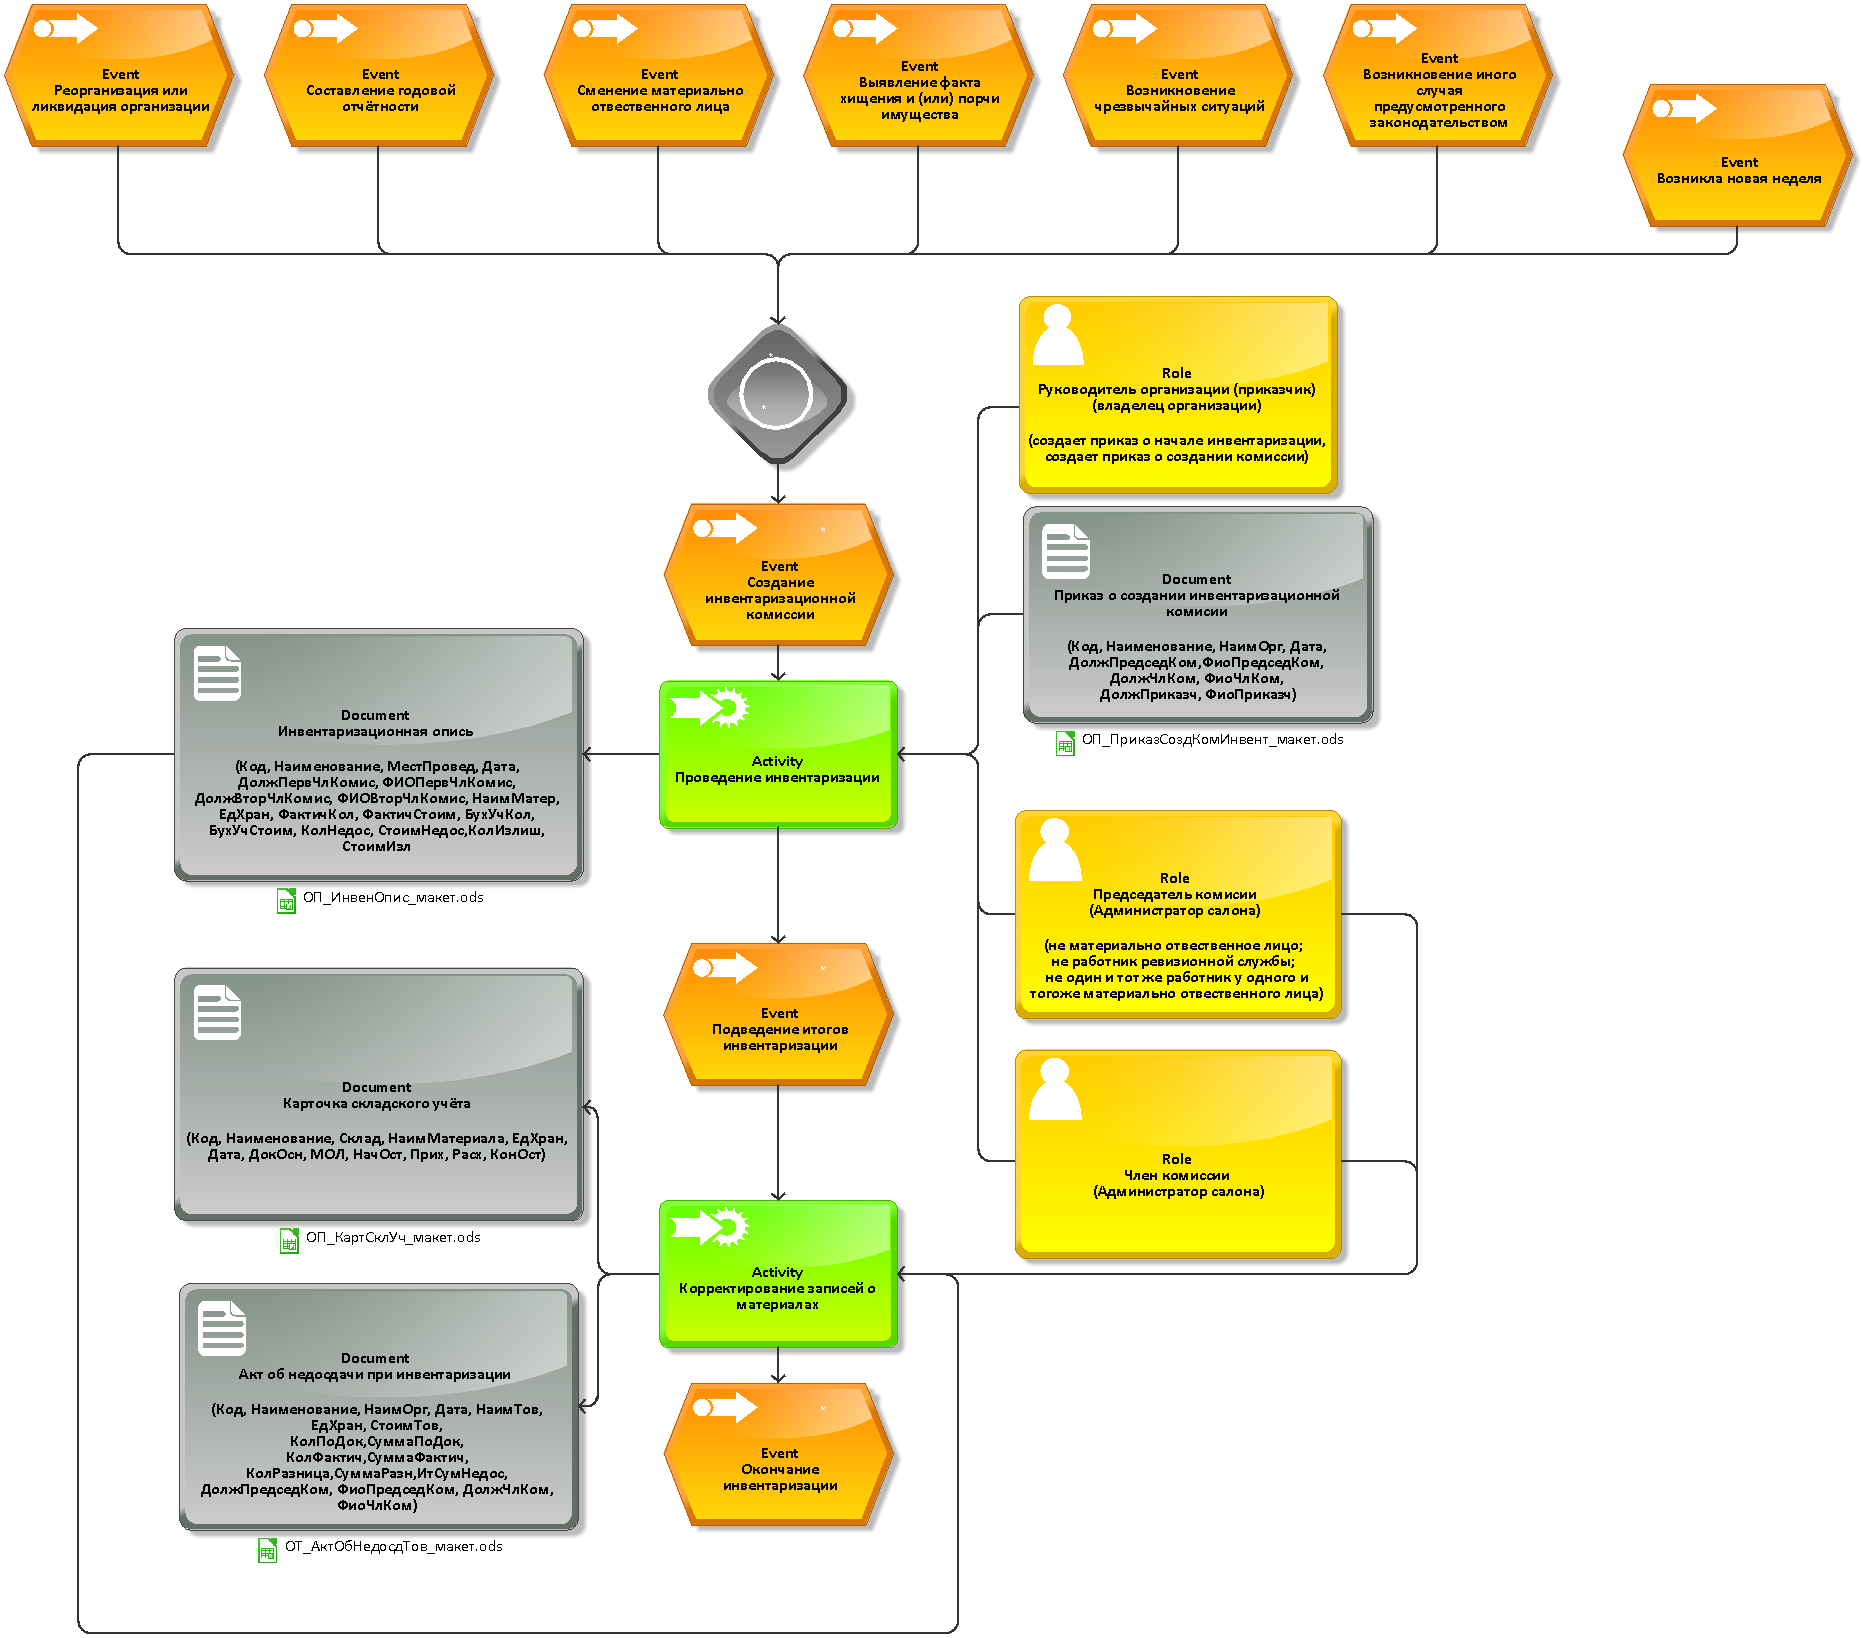
\includegraphics[width=18cm]
            {_docs/БизнесМодельИнвентаризация.png}
        \caption{Бизнес модель инвентаризации}
        \label{fig:BusinessModelInvent}
    \end{figure}

    % = = = = = = = = = = = = = = = =
    \newpage
    \section{РАЗРАБОТКА БАЗЫ ДАННЫХ}
    \subsection{Концептуальная модель}

    Предметная область - совокупность объектов,
    свойства которых и отношения между которыми рассматриваются в рамках некоторого исследования.
    
    Модель предметной области – некоторая система, адекватно имитирующая
    структуру и функционирование исследуемой предметной области.

    Концептуальная модель - это структура моделируемой предметной области,
    свойств её элементов и причинно-следственных связей, присущих системе и
    существенных для достижения цели моделирования.
    В рамках этапа концептуального моделирования выделяются основные смысловые единицы (сущности)
    предметной области, определяются и описываются связи между ними.
    
    Концептуальная модель ориентирована на потенциальных пользователей базы данных,
    так как представляет предметную область на их уровне понимания.
    Этот уровень называется системно-независимым или предметно-ориентированным.
    
    \subsubsection{ЛКМ для БП <<Приказ о создании комиссии инвентаризационной>>}

    Локальная концептуальная модель для бизнес процесса с документом <<Приказ о создании комиссии инвентаризационной>>
    изображена на рисунке~\ref{fig:LKM_PrikazSozdKomInvent}.

    \begin{figure}[!h]
        \centering
        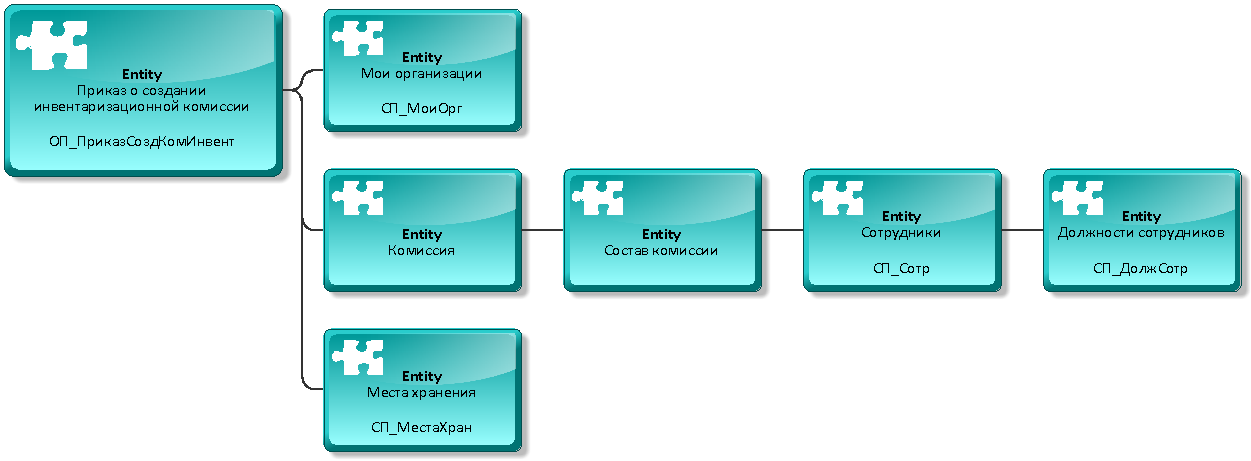
\includegraphics[width=18cm]
            {_docs/ЛКМ_ПриказСоздКомИнвент.png}
        \caption{Локальная концептуальная модель для бизнес процесса с документом <<Приказ о создании комиссии инвентаризационной>>}
        \label{fig:LKM_PrikazSozdKomInvent}
    \end{figure}

    \subsubsection{ЛКМ для БП <<Инвентаризационная опись>>}

    Локальная концептуальная модель для бизнес процесса с документом <<Инвентаризационная опись>>
    изображена на рисунке~\ref{fig:LKM_InvenOpis}.

    \begin{figure}[!h]
        \centering
        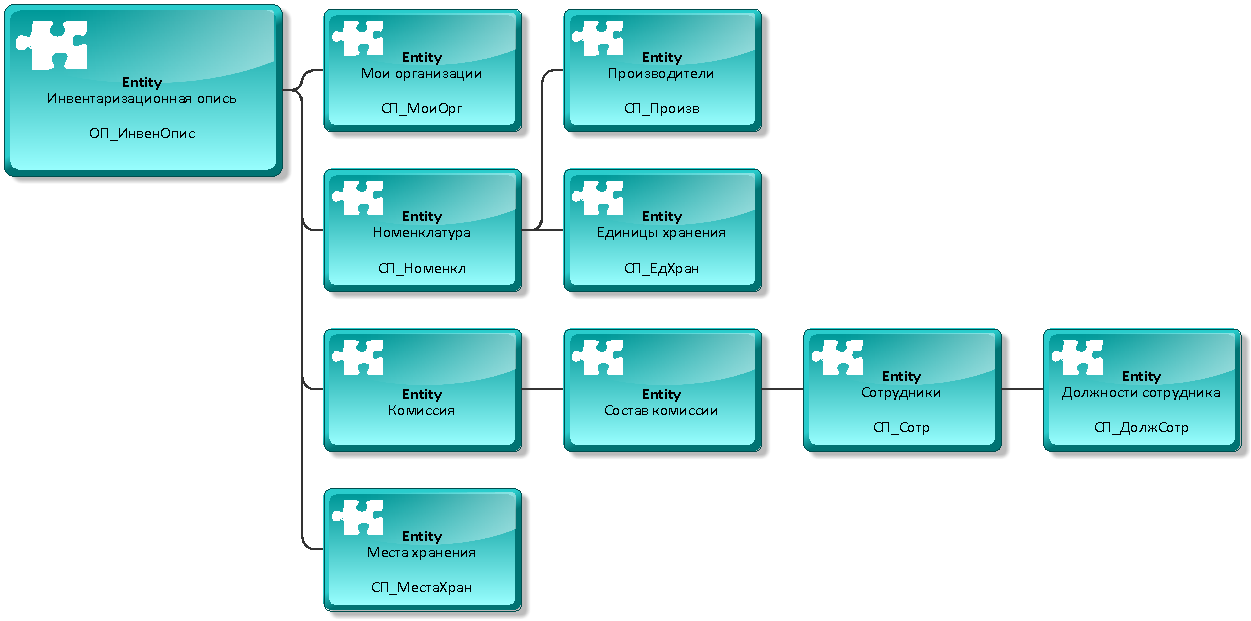
\includegraphics[width=18cm]
            {_docs/ЛКМ_ИнвенОпис.png}
        \caption{Локальная концептуальная модель для бизнес процесса с документом <<Инвентаризационная опись>>}
        \label{fig:LKM_InvenOpis}
    \end{figure}

    \subsubsection{Общая концептуальная модель}

    Общая концептуальная подель процесса <<Инвентаризация>>
    изображена на рисунке~\ref{fig:KP}.

    \begin{figure}[!hp]
        \centering
        \includegraphics[width=18cm]
            {_docs/КМ.png}
        \caption{Общая концептуальная модель}
        \label{fig:KP}
    \end{figure}

    \newpage
    \subsection{Логическая модель}

    \newpage
    \subsection{Физическая модель}

    %
    \newpage
    \addcontentsline{toc}{section}{ЗАКЛЮЧЕНИЕ}
    \section*{ЗАКЛЮЧЕНИЕ}
    \newpage

    %
    \newpage
    \addcontentsline{toc}{section}{СПИСОК ИСПОЛЬЗОВАННЫХ ИСТОЧНИКОВ}
    \section*{СПИСОК ИСПОЛЬЗОВАННЫХ ИСТОЧНИКОВ}
    \begin{enumerate}    
        \item[1.] Форма 401 1. Приложение 5. 2. к Инструкции по...
        - [Электронный ресурс]
        Режим доступа: \url{https://neg.by/public_files/NEG__5.XLS}
        Дата~доступа:~08.03.2022.
        \item[2.] Годовая инвентаризация 2021 (Как проводится инвентаризация)
        - [Электронный ресурс]
        Режим доступа: \url{https://www.gb.by/articles/godovaya-inventarizatsiya-2020}
        Дата~доступа:~15.03.2022.
        \item[3.] 10.docx (Приказ о назначении инвентаризационной комиссии)
        - [Электронный ресурс]
        Режим доступа: \url{https://docviewer.yandex.by/view/0/?*=bRCKBHW0FptcY0rJ%2BVjcsYyxekV7InVybCI6Imh0dHBzOi8vanVyYnVoLmJ5L2RvY3Mvb3JkZXJzLzEwLmRvY3giLCJ0aXRsZSI6IjEwLmRvY3giLCJub2lmcmFtZSI6dHJ1ZSwidWlkIjoiMCIsInRzIjoxNjQ3Mzc2NzAyMjQwLCJ5dSI6IjUyNTIwNjUwMjE2NDQ3NTk1NzciLCJzZXJwUGFyYW1zIjoidG09MTY0NzM3NjY4MyZ0bGQ9YnkmbGFuZz1ydSZuYW1lPTEwLmRvY3gmdGV4dD0lRDAlQkYlRDElODAlRDAlQjglRDAlQkElRDAlQjAlRDAlQjcrJUQwJUJFKyVEMSU4MSVEMCVCRSVEMCVCNyVEMCVCNCVEMCVCMCVEMCVCRCVEMCVCOCVEMCVCOCslRDAlQkElRDAlQkUlRDAlQkMlRDAlQjglRDElODElRDElODElRDAlQjglRDAlQjgrJUQwJUI4JUQwJUJEJUQwJUIyJUQwJUI1JUQwJUJEJUQxJTgyJUQwJUIwJUQxJTgwJUQwJUI4JUQwJUI3JUQwJUIwJUQxJTg2JUQwJUI4JUQwJUJFJUQwJUJEJUQwJUJEJUQwJUJFJUQwJUI5JnVybD1odHRwcyUzQS8vanVyYnVoLmJ5L2RvY3Mvb3JkZXJzLzEwLmRvY3gmbHI9MjE1MTAmbWltZT1kb2N4JmwxMG49cnUmc2lnbj1jNzE4NzE4YWYzNWI3MDkyOGViYTcyOWI2ZTY5OTAzNyZrZXlubz0wIn0%3D&amp;lang=ru}
        Дата~доступа:~15.03.2022.
    \end{enumerate}
    \newpage

    %
    \newpage
    \addcontentsline{toc}{section}{СПИСОК СОКРАЩЕНИЙ}
    \section*{СПИСОК СОКРАЩЕНИЙ}
    
    \begin{tabular}{ll} 
        ARIS    & architecture of integrated information system.\\
        ИС      & информационная система.\\
        МОЛ     & материально отвественное лицо.\\
        ОА      & объект автоматизации.\\
        ОП      & оперативный документ.\\
        ОТ      & отчётный документ.\\
        СП      & справочный документ.\\
        % СУБД    & система управления базами данных.\\
        % ТМЦ     & товарно-материальные ценности.\\
        БД      & база данных.\\
        ЛКМ     & локальная концептуальная модель \\ 
        КМ      & концептуальная модель \\
    \end{tabular}
    
    \newpage
\end{document}
